\documentclass{article}

\usepackage{graphicx}
\usepackage[utf8]{inputenc}
\usepackage[english]{babel}
\usepackage[document]{ragged2e}
\usepackage{geometry}
 \geometry{
 a4paper,
 total={170mm,257mm},
 left=20mm,
 top=20mm,
 }


\begin{document}
{\textbf{CS663: Assignment 4 - Q1}}
\vskip 0.2in

Pranav Sankhe \\ Kalpesh Krishna \\ Mohit Madan 

\vskip 0.5in
Implemented a mini face recognition system using PCA.

\vskip 0.2in

\textbf{Results on ORL Face Dataset}

\vskip 0.5in
Applying PCA by computing eigenvectors of the covariance matrix
\begin{figure}[h!]
  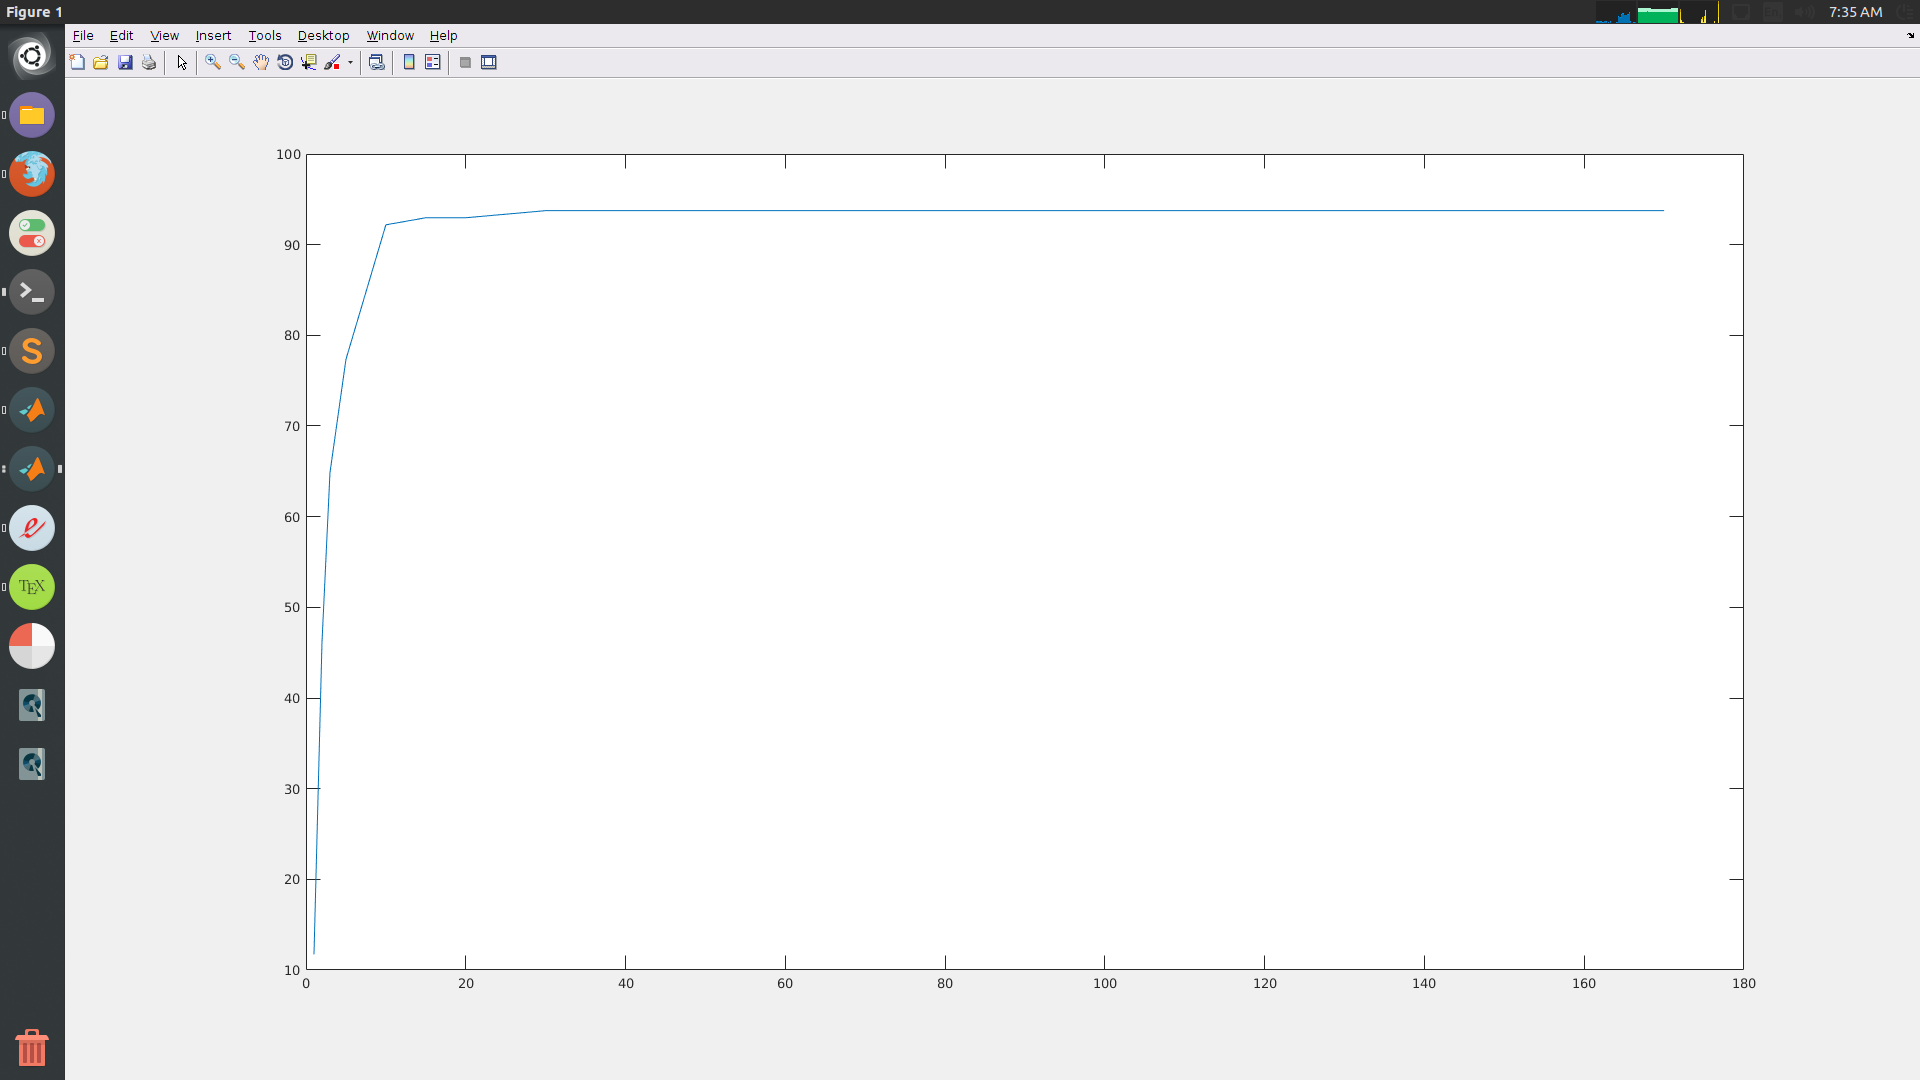
\includegraphics[width=\linewidth]{Q1cov.png}
  \caption{Recognition rate vs k(no. of principal components)}
  \label{fig:result1}
\end{figure}
\newpage
Applying PCA using Singular Value Decomposition (SVD)
\begin{figure}[h!]
  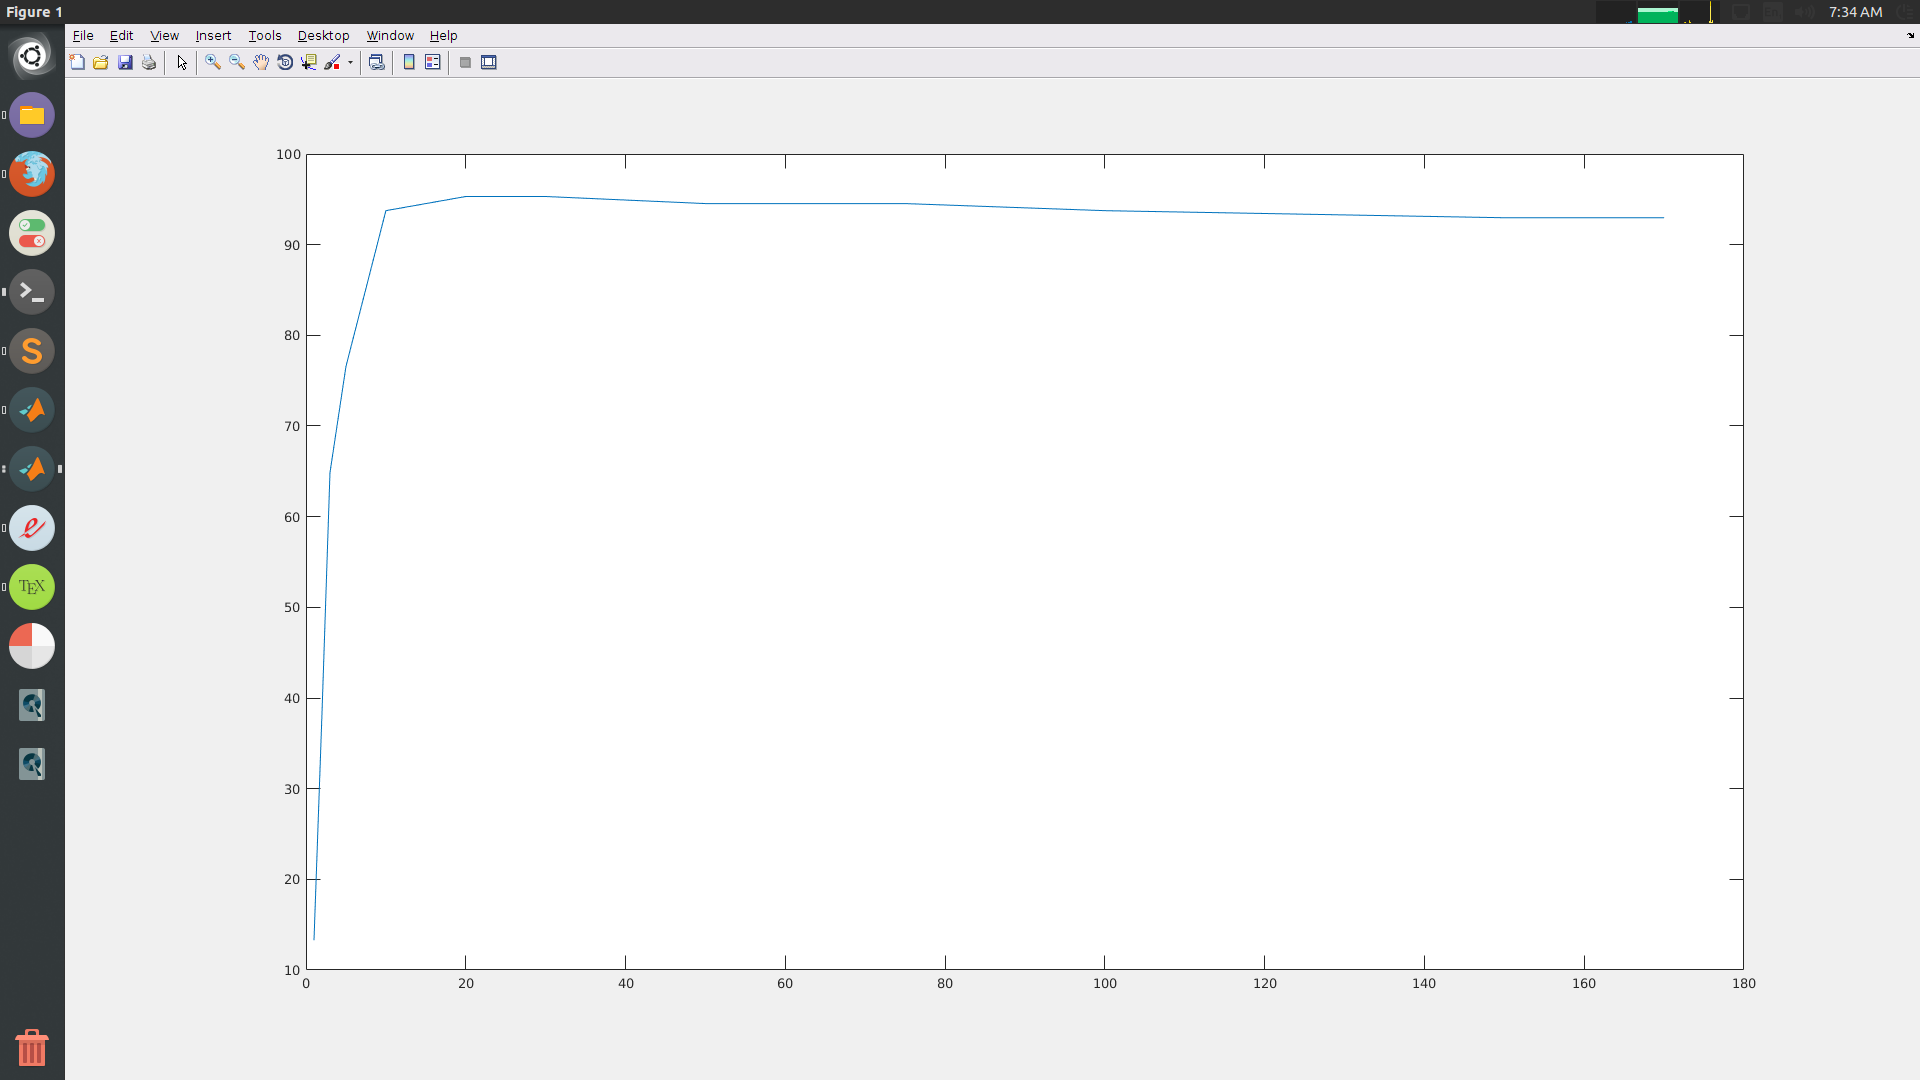
\includegraphics[width=\linewidth]{Q1_svd.png}
  \caption{Recognition rate vs k(no. of principal components)}
  \label{fig:result2}
\end{figure}

\newpage

\textbf{Results on Yale Dataset}
\vskip 0.5in

Applying PCA using Singular Value Decomposition (SVD)  comparing the results if we ignore the first three eigenvectors which correspons to maximum variance in the dataset in order to analyse the effect of ilumination conditions and how can we mitigate these effects. 
We cam clearly see that by ignoring the first three eigenfaces, the recognition accuracy has increasesd.  
\begin{figure}[h!]
  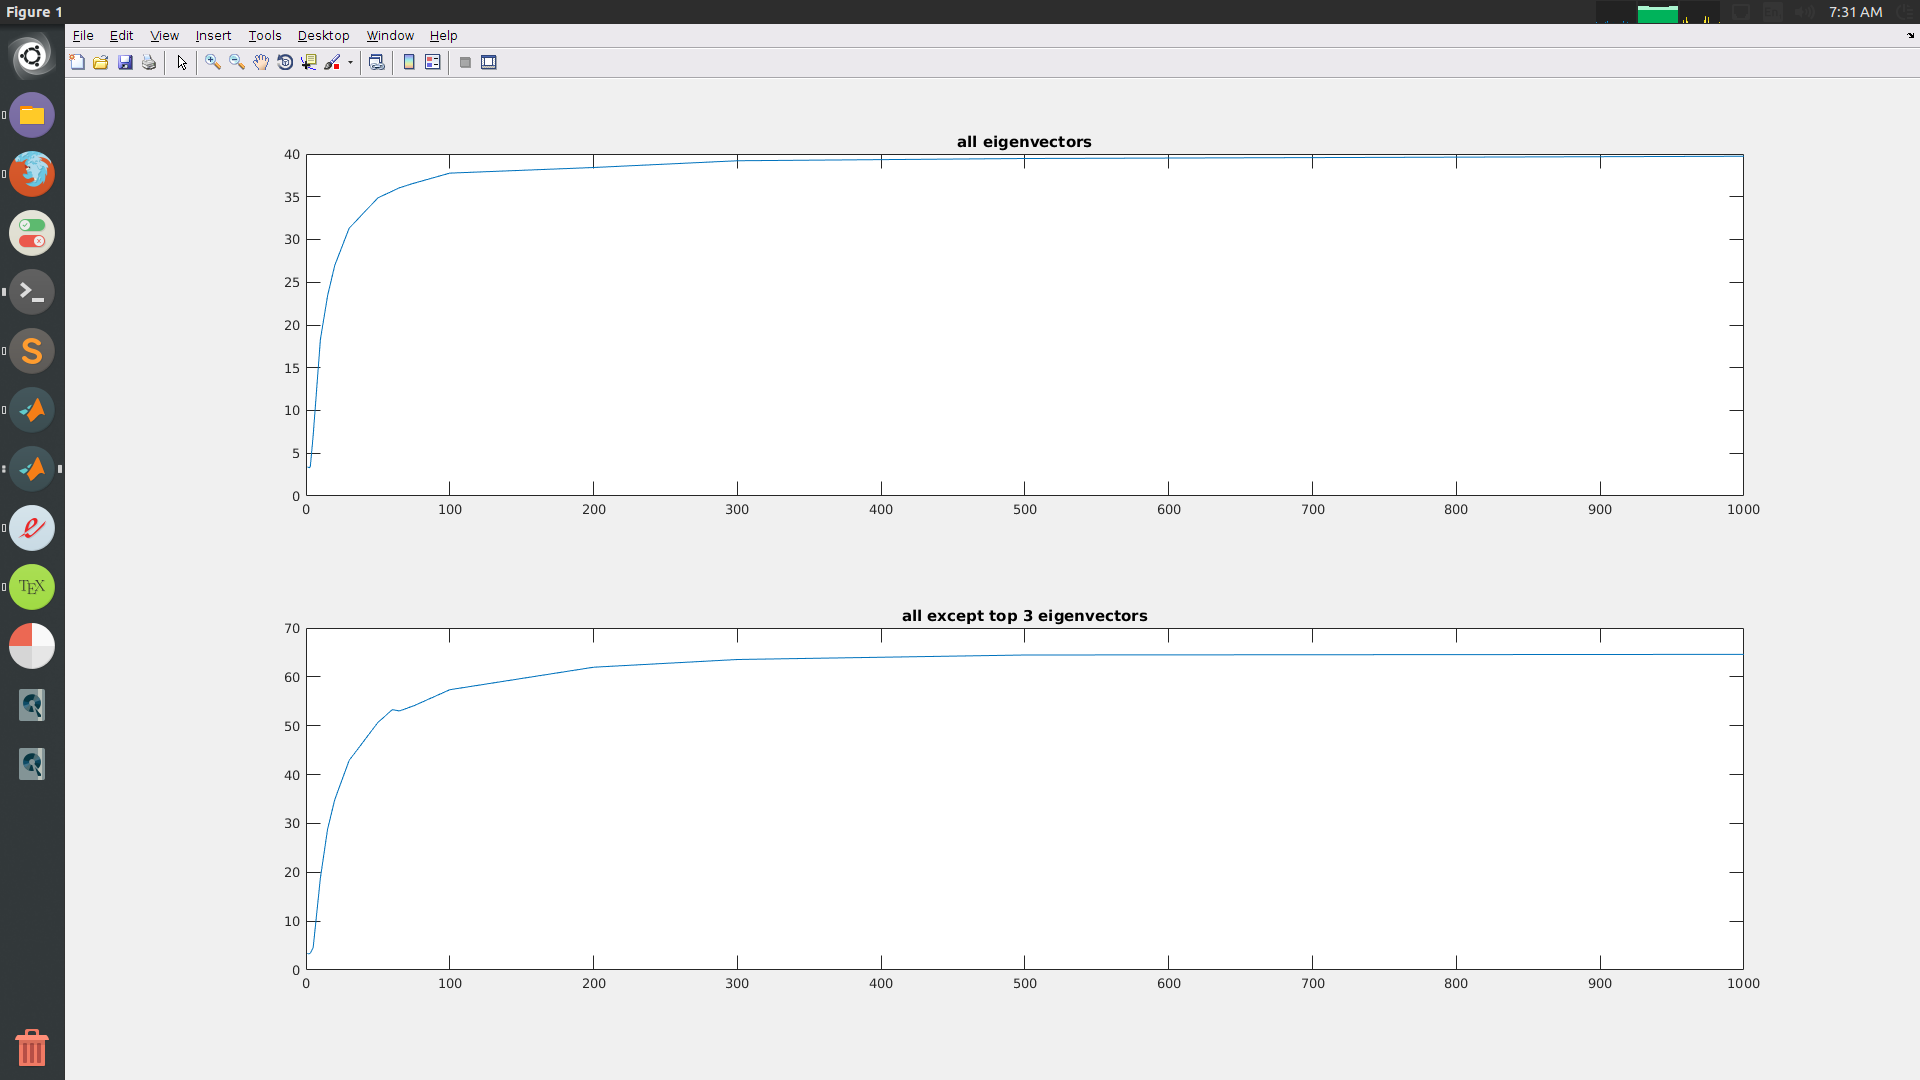
\includegraphics[width=\linewidth]{Q1_yale.png}
  \caption{Recognition rate vs k(no. of principal components)}
  \label{fig:result2}
\end{figure}
\end{document}